%! TEX root = main.tex

\graphicspath{{00_Images/07_chapter/}}

\chapter{Transistors and Active Components}
\label{ch:transistors}

\section{Introduction to Active Elements}
\label{sc:71}

Every operational amplifier examined in the preceding chapters is itself built from active semiconductor devices: the external black-box model of infinite input impedance and voltage controlled output is a macroscopic description of an internal network of transistors or, in older high-voltage designs, thermionic valves (tubes).
Understanding the behavior of these underlying devices is essential for appreciating the limits of real OPAMPs, for designing discrete amplifier stages, and for analyzing the practical circuits encountered throughout audio electronics.
Active devices are classified into two broad families, each exploiting a distinct physical mechanism to achieve power gain.
Bipolar Junction Transistors (BJT) control output current by means of an input current: the collector current is an exponential function of the base-emitter voltage and simultaneously a linear function of the base current through the current gain \(\beta\).
Field Effect Transistors (FET) control output current by means of an input voltage applied to an electrically insulated or reverse-biased gate terminal, so that the gate draws essentially no current and the input impedance is ideally infinite.
The FET family is further divided into two distinct types.
A Junction FET (JFET) uses a reverse-biased pn junction to form a depletion region that modulates the width of the conducting channel; it is a normally-on device that is pinched off by a sufficiently large reverse gate voltage.
A Metal-Oxide Semiconductor FET (MOSFET) separates the gate electrode from the semiconductor channel by a thin oxide insulating layer, achieving an even higher input impedance; both types can be realized as n-channel or p-channel devices, giving rise to complementary pairs widely used in integrated circuit design.

\begin{figure}[!htb]
    \centering
    \subfloat[NPN BJT: Base (B), Collector (C), Emitter (E)]{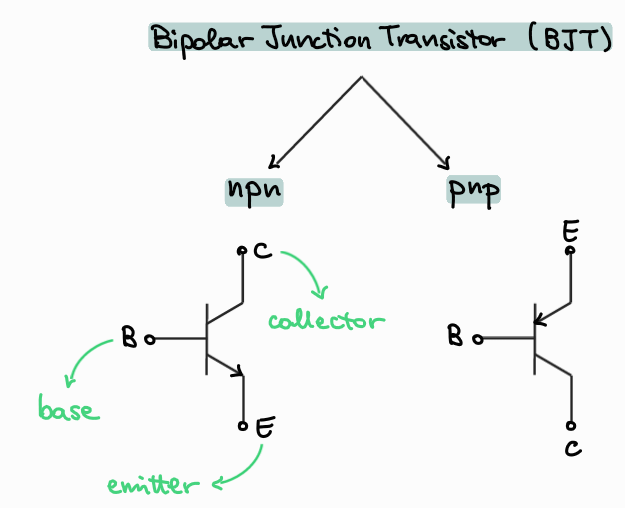
\includegraphics[height=0.18\textheight]{BJT_Symbole.png}}
    \hfill
    \subfloat[nMOS and pMOS: Gate (G), Drain (D), Source (S)]{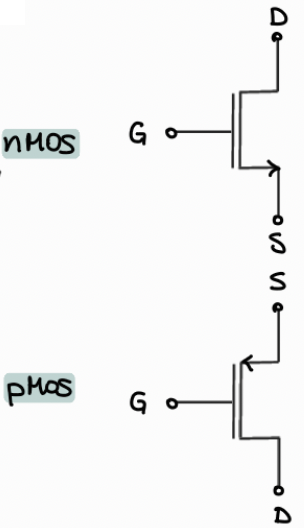
\includegraphics[height=0.18\textheight]{NMOS_PMOS.png}}
    \hfill
    \subfloat[JFET: Gate (G), Drain (D), Source (S)]{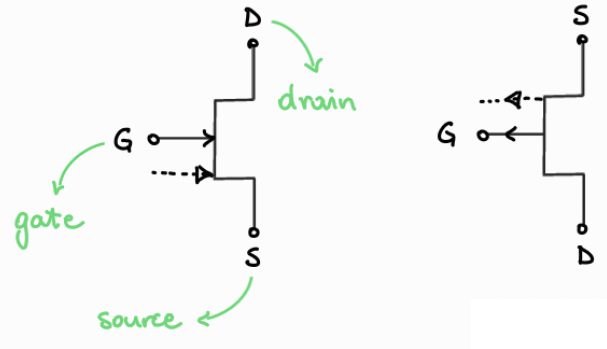
\includegraphics[height=0.18\textheight]{JFET.png}}
    \caption{Circuit symbols and terminal labeling for the three main transistor families: BJT, MOSFET, and JFET}
    \label{fig:transistorSymbols}
\end{figure}

\section{Operating Regions and Large-Signal Equations}
\label{sc:72}

The three device families share a common terminal naming convention for their output port: current flows from Collector to Emitter in a BJT, and from Drain to Source in any FET variant.
The controlling terminal is the Base in a BJT and the Gate in all FETs.
Each device exhibits three operating regions, corresponding to qualitatively different circuit behaviors.

\subsection{Off-State (Cutoff)}
\label{ssc:721}

In the off-state the controlling terminal voltage is insufficient to establish a conducting path and the output current is negligibly small.
For the BJT, cutoff occurs when \(v_{BE} < \SI{0.5}{\volt}\), leaving the base-emitter junction unbiased and giving \(i_C \approx 0\).
For the n-channel MOSFET, the condition is \(v_{GS} < V_{TH}\), where the threshold voltage \(V_{TH}\) is a technology parameter in the range \SI{0.4}{\volt} to \SI{1.5}{\volt}; below this threshold \(i_D = 0\) because no inversion channel forms under the gate oxide.
The JFET operates in the opposite sense: it is a normally-on device that carries its maximum drain current when \(v_{GS} = 0\) and is turned off only when the gate voltage reaches the pinch-off value \(V_P < 0\), at which point the channel is fully depleted.

\subsection{Active Region (Amplification)}
\label{ssc:722}

The active region is the zone in which each device operates as a voltage-controlled current source, producing an output current that is a smooth, differentiable function of the input voltage.
This is the region used for linear signal amplification, because the nonlinear large-signal characteristic can be linearized around a stable DC operating point.
For the BJT the active region requires \(v_{BE} \geq \SI{0.7}{\volt}\) and \(v_{CE} \geq \SI{0.2}{\volt}\).
The collector current obeys the exponential Shockley law
\[
i_C = I_s \, e^{v_{BE}/V_T}
\]
where \(V_T \approx \SI{26}{\milli\volt}\) at room temperature is the thermal voltage, and the simultaneous current gain relation
\[
i_C = \beta \, i_B, \qquad \beta \in [50, 300]
\]
yields \(i_E = (\beta + 1)i_B \approx i_C\) for \(\beta \gg 1\).
For the n-channel MOSFET the active (saturation) region requires \(v_{GS} > V_{TH}\) and \(v_{DS} \geq V_{OV} = v_{GS} - V_{TH}\); the drain current follows the quadratic law
\[
i_D = k(v_{GS} - V_{TH})^2
\]
with \(i_G \approx 0\) because the oxide layer provides a capacitive barrier.
For the JFET in saturation (\(v_{DS} \geq V_{OV}\)):
\[
i_D = k \left(1 - \frac{v_{GS}}{V_P}\right)^2
\]
with \(i_G \approx 0\) and \(r_{in} \to \infty\).

\subsection{Varistor Region (Low Output Voltage)}
\label{ssc:723}

When the voltage across the output terminals falls below a device-specific threshold, the device leaves the active region and enters a zone in which the output current is no longer independent of the output voltage: it behaves as a variable resistor (varistor).
For the BJT this is called the saturation region (\(v_{CE} < \SI{0.2}{\volt}\)), where the collector-emitter path presents a small resistance \(R_{sat} = v_{CE}/i_C\) of typically a few ohms.
For the MOSFET and JFET the equivalent zone is called the triode region (\(v_{DS} < V_{OV}\)), where the drain-source conductance depends on both \(v_{GS}\) and \(v_{DS}\).

\begin{figure}[!htb]
    \centering
    \subfloat[\(i_C(v_{CE})\) characteristic of the BJT: cutoff, active, and saturation regions]{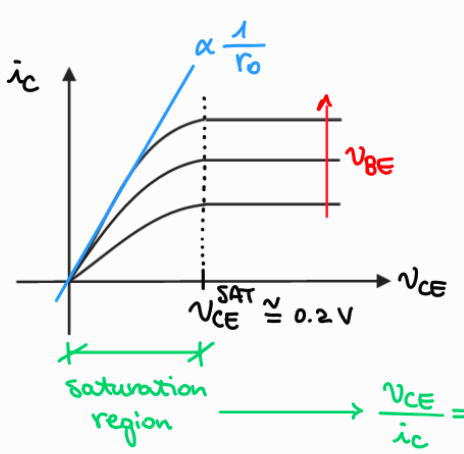
\includegraphics[height=0.22\textheight]{BJT_Varistor.png}}
    \hfill
    \subfloat[\(i_D(v_{DS})\) characteristic of the nMOSFET: off, triode, and saturation regions]{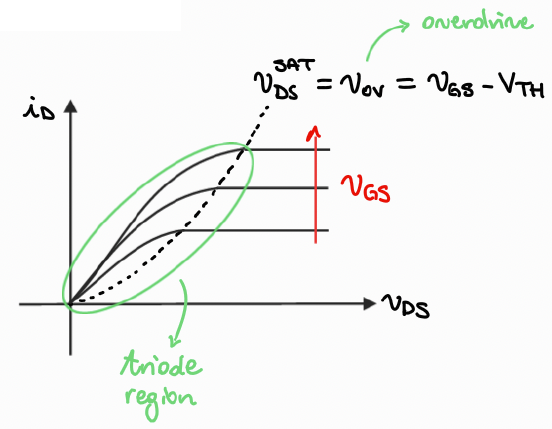
\includegraphics[height=0.22\textheight]{nMOS_Varistor.png}}
    \caption{Output characteristic curves illustrating the three operating regions for BJT (left) and MOSFET (right)}
    \label{fig:operatingRegions}
\end{figure}

\section{The Small-Signal Model}
\label{sc:73}

The large-signal equations of section \ref{sc:72} are nonlinear and cannot be analyzed directly with the superposition, Thevenin, and Laplace techniques developed in chapter \ref{ch:rev}.
The standard approach is to establish a DC operating point (Q-point) by choosing suitable bias voltages, then restrict analysis to small AC signals superimposed on that bias.
Within the neighborhood of the Q-point the nonlinear characteristic is approximated by its first-order Taylor expansion, yielding a linear small-signal model valid for small-amplitude excitation.

\subsection{Transconductance}
\label{ssc:731}

The transconductance \(g_m\) is the conversion factor from a small AC input voltage to a small AC output current; it is the derivative of the output current with respect to the input voltage, evaluated at the Q-point.

\paragraph{BJT derivation} Writing \(v_{BE} = V_{BE}^{OP} + v_{be}\) with \(|v_{be}| \ll V_T\), the first-order Taylor expansion of the exponential collector current law gives the small-signal collector current
\[
i_c = g_m v_{be}, \qquad g_m = \frac{I_C}{V_T}
\]
The transconductance is proportional to the quiescent collector current: a higher bias yields a stiffer \(g_m\).
For a typical operating point with \(I_C = \SI{330}{\micro\ampere}\), \(g_m = 330/26 \approx \SI{13}{\milli\siemens}\).

\paragraph{MOSFET and JFET derivation} Applying the same linearization to the quadratic drain current law:
\[
g_m = 2k(V_{GS}^{OP} - V_{TH}) = 2\sqrt{k \cdot I_D}
\]
The JFET transconductance has the identical form \(g_m = 2\sqrt{k \cdot I_D}\).

\subsection{Input Resistance}
\label{ssc:732}

The small-signal input resistance seen at the controlling terminal determines how much the transistor loads the driving stage.

\paragraph{BJT} The base draws current \(i_b = i_c/\beta = (g_m/\beta)v_{be}\), giving the small-signal base-emitter resistance
\[
r_\pi = \frac{v_{be}}{i_b} = \frac{\beta}{g_m} = \frac{\beta V_T}{I_C}
\]
For the numerical example above, \(r_\pi = 300/\SI{13}{\milli\siemens} \approx \SI{22}{\kilo\ohm}\).

\paragraph{MOSFET and JFET} The gate draws no current because the oxide layer or the reverse-biased junction prevents DC conduction, so the small-signal gate current is \(i_G \approx 0\) and the input impedance is ideally infinite: \(r_{in} \to \infty\).
This property makes FETs intrinsically superior to BJTs whenever the source impedance is high, because they impose virtually no loading on the preceding stage.

\begin{figure}[!htb]
    \centering
    \subfloat[Simplified small-signal model: \(g_m v_{be}\) controlled source]{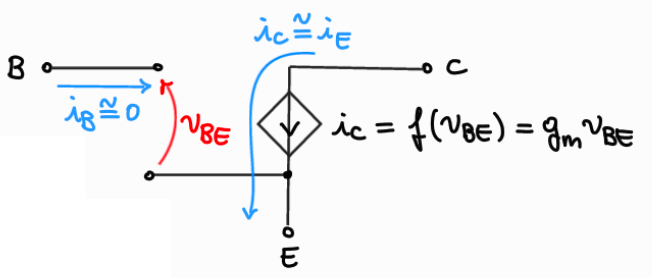
\includegraphics[width=0.45\linewidth]{BJT_Simple_Equiv_Scheme.png}}
    \hfill
    \subfloat[Complete hybrid-\(\pi\) model with \(r_\pi\), \(g_m v_{be}\), and \(r_0\)]{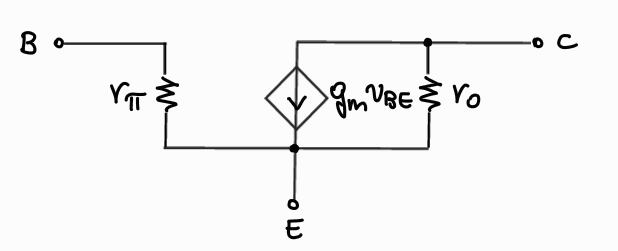
\includegraphics[width=0.45\linewidth]{BJT_Complete_Scheme.png}}
    \caption{Small-signal models of the BJT in the active region: simplified approximation (left) and complete hybrid-\(\pi\) equivalent (right)}
    \label{fig:hybridPi}
\end{figure}

In the complete hybrid-\(\pi\) model of figure \ref{fig:hybridPi}, the input port consists of \(r_\pi\) between base and emitter, and the output port is represented by the controlled current source \(g_m v_{be}\) in parallel with the output resistance \(r_0 = \partial v_{CE}/\partial i_C\).
In the ideal model \(r_0 \to \infty\) and the collector behaves as a perfect current source; in practice \(r_0 \approx \SI{100}{\kilo\ohm}\) due to the Early effect, where the effective base width is modulated by \(v_{CE}\).
An analogous model applies to FETs with \(v_{gs}\) replacing \(v_{be}\) and \(r_{in} \to \infty\) at the gate terminal.

\section{The Emitter Follower (Voltage Buffer)}
\label{sc:74}

The emitter follower, also called the common-collector configuration, is the discrete BJT realization of a voltage buffer: a stage with unity voltage gain, very high input impedance, and very low output impedance, which transfers a signal from a high-impedance source to a low-impedance load without attenuation.
In this topology the collector is connected to the supply rail \(V_{CC}\) (AC short circuit to ground), the input signal is applied to the base, and the output is taken from the emitter through the load resistance \(R_L\) to ground.

\begin{figure}[!htb]
    \centering
    \subfloat[DC circuit: emitter follower with load \(R_L\)]{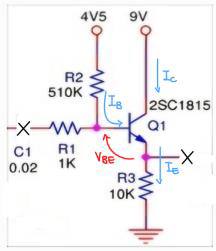
\includegraphics[height=0.22\textheight]{Tube_Screamer_Common_Collector_1.png}}
    \hspace{1.5cm}
    \subfloat[AC small-signal equivalent used to derive \(Z_{in}\) and \(A_V\)]{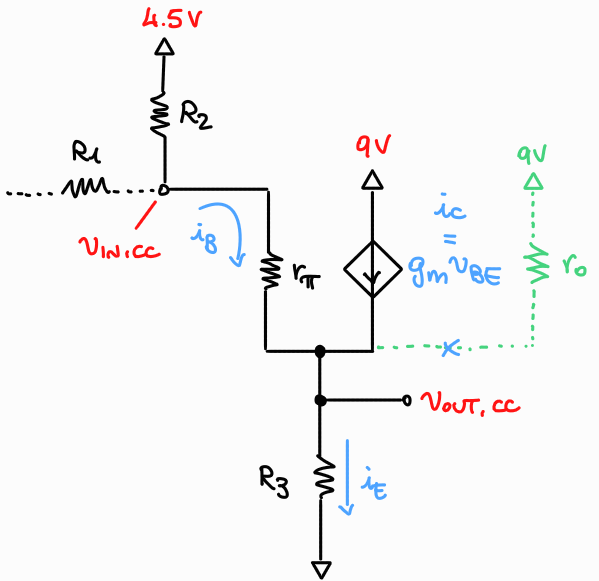
\includegraphics[height=0.22\textheight]{Tube_Screamer_Common_Collector_1_equiv_scheme.png}}
    \caption{Emitter follower (common-collector): DC circuit and small-signal AC equivalent used for the input impedance and voltage gain derivation}
    \label{fig:emitterFollower}
\end{figure}

\subsection{Input Impedance Derivation}
\label{ssc:741}

Replacing the BJT with its hybrid-\(\pi\) model and setting the supply to zero for AC analysis, the small-signal equivalent circuit has \(r_\pi\) between base and emitter, the controlled source \(g_m v_{be}\) from collector (grounded) to emitter, and \(R_L\) from emitter to ground.
KVL around the input loop, with \(i_E = (\beta+1)i_B\) from KCL, gives
\[
v_{in} = i_B r_\pi + i_E R_L = i_B r_\pi + (\beta+1)i_B R_L
\]
and the input impedance looking into the base is therefore
\[
Z_{in} = \frac{v_{in}}{i_B} = r_\pi + (\beta+1)R_L
\]
The load resistance \(R_L\) at the emitter is seen from the base magnified by \((\beta+1)\): for \(\beta = 300\) and \(R_L = \SI{10}{\kilo\ohm}\), \(Z_{in} = \SI{22}{\kilo\ohm} + 301 \times \SI{10}{\kilo\ohm} \approx \SI{3}{\mega\ohm}\), negligibly loading any practical preceding stage.

\subsection{Voltage Gain}
\label{ssc:742}

Using \(v_{be} = v_{in} - v_{out}\) from KVL and \(i_E \approx i_C = g_m v_{be}\):
\[
v_{out} = g_m R_L(v_{in} - v_{out}) \quad \Rightarrow \quad v_{out}(1 + g_m R_L) = g_m R_L \, v_{in}
\]
\[
A_V = \frac{v_{out}}{v_{in}} = \frac{g_m R_L}{1 + g_m R_L} \approx 1 \qquad \text{when } g_m R_L \gg 1
\]
For the example values \(g_m R_L = \SI{13}{\milli\siemens} \times \SI{10}{\kilo\ohm} = 130 \gg 1\), giving \(A_V = 130/131 \approx 0.99\), confirming near-unity voltage gain.
The emitter follower provides no voltage amplification but delivers substantial current amplification: the source drives only the base current \(i_B\), while the load receives the emitter current \(i_E = (\beta+1)i_B\), amplified by the factor \((\beta+1) \approx 300\).
The output impedance seen looking into the emitter with the base driven from a source of resistance \(R_B\) is
\[
Z_{out} = \frac{R_B + r_\pi}{\beta+1} \approx \frac{1}{g_m}
\]
which is very low, of the order of tens to hundreds of ohms, enabling the stage to drive reactive or low-impedance loads without signal degradation.
This buffering mechanism is the same principle exploited in the Class A power amplifier output stage discussed in section \ref{ssc:121}, where the emitter follower topology delivers the current required by the loudspeaker while preserving the voltage set by the preceding preamplifier chain.